% **************************************************
% Document Class Definition
% **************************************************
\documentclass[%
    paper=A4,               % paper size --> A4 is default in Germany
    twoside=true,           % onesite or twoside printing
    openright,              % doublepage cleaning ends up right side
    parskip=half,           % spacing value / method for paragraphs
    chapterprefix=true,     % prefix for chapter marks
    11pt,                   % font size
    headings=normal,        % size of headings
    bibliography=totoc,     % include bib in toc
    listof=totoc,           % include listof entries in toc
    titlepage=on,           % own page for each title page
    captions=tableabove,    % display table captions above the float env
    chapterprefix=false,    % do not display a prefix for chapters
    appendixprefix=false,    % but display a prefix for appendix chapter
    draft=false,            % value for draft version
]{scrreprt}%


% **************************************************
% Setup YOUR thesis document in this file !
% **************************************************

% **************************************************
% Files' Character Encoding
% **************************************************
\PassOptionsToPackage{utf8}{inputenc}
\usepackage{inputenc}


% **************************************************
% Information and Commands for Reuse
% **************************************************
\newcommand{\thesisTitle}{Xiang Li's Thesis title}
\newcommand{\thesisName}{Xiang Li}
\newcommand{\thesisSubject}{My Subject}
\newcommand{\thesisDate}{June 21, 2022}
\newcommand{\thesisVersion}{My First Draft}

\newcommand{\thesisFirstReviewer}{Jane Doe}
\newcommand{\thesisFirstReviewerUniversity}{\protect{Clean Thesis Style University}}
\newcommand{\thesisFirstReviewerDepartment}{Department of Clean Thesis Style}

\newcommand{\thesisSecondReviewer}{John Doe}
\newcommand{\thesisSecondReviewerUniversity}{\protect{Clean Thesis Style University}}
\newcommand{\thesisSecondReviewerDepartment}{Department of Clean Thesis Style}

\newcommand{\thesisFirstSupervisor}{Jane Doe}
\newcommand{\thesisSecondSupervisor}{John Smith}

\newcommand{\thesisUniversity}{\protect{Queen's University Belfast}}
\newcommand{\thesisUniversityDepartment}{Arts, Humanities And Social Sciences}
\newcommand{\thesisUniversityInstitute}{School of Arts, English and Languages (AEL)}
\newcommand{\thesisUniversityGroup}{Clean Thesis Group (CTG)}
\newcommand{\thesisUniversityCity}{City}
\newcommand{\thesisUniversityStreetAddress}{Street address}
\newcommand{\thesisUniversityPostalCode}{Postal Code}


% **************************************************
% Debug LaTeX Information
% **************************************************
%\listfiles


% **************************************************
% Load and Configure Packages
% **************************************************
\usepackage[english]{babel} % babel system, adjust the language of the content
\PassOptionsToPackage{% setup clean thesis style
    figuresep=colon,%
    hangfigurecaption=false,%
    hangsection=true,%
    hangsubsection=true,%
    sansserif=false,%
    configurelistings=true,%
    colorize=full,%
    colortheme=bluemagenta,%
    configurebiblatex=true,%
    bibsys=biber,%
    bibfile=bib-refs,
    % your bib file name withoud extension .bib
    bibstyle=alphabetic,
    % alphabetic: authoryear like [Lan+15] or [LHD17]
    % numeric: numeric labels, such as [1] or [37]
    bibsorting=nty,
    % nty: sort by name, title, year
    % nyt: sort by name, year, title
    % none: sort in the order of citation
}{cleanthesis}
\usepackage{usercommand}
\usepackage{cleanthesis}
\hypersetup{% setup the hyperref-package options
    pdftitle={\thesisTitle},    %   - title (PDF meta)
    pdfsubject={\thesisSubject},%   - subject (PDF meta)
    pdfauthor={\thesisName},    %   - author (PDF meta)
    plainpages=false,           %   -
    colorlinks=false,           %   - colorize links?
    pdfborder={0 0 0},          %   -
    breaklinks=true,            %   - allow line break inside links
    bookmarksnumbered=true,     %
    bookmarksopen=true          %
}


\makenoidxglossaries
\setacronymstyle{long-short}

\newacronym{acc}{ACC}{acoustic contrast control}
\newacronym{chdacc}{CHDACC}{circular harmonic domain acoustic contrast control}
\newacronym{shdacc}{SHDACC}{spherical harmonic domain acoustic contrast control}
\newacronym{pm}{PM}{pressure matching}
\newacronym{mm}{MM}{mode matching}
\newacronym{wmm}{WMM}{weighted mode matching}
\newacronym{bc}{BC}{brightness control}
\newacronym{aed}{AED}{acoustic energy difference}
\newacronym{jpvm}{JPVM}{joint pressure and velocity matching}
\newacronym{pc}{PC}{planarity control}
\newacronym{wco}{WCO}{worst case optimization}
\newacronym{ac}{AC}{acoustic contrast}
\newacronym{ag}{AG}{array gain}
\newacronym{dft}{DFT}{discrete Fourier transform}
\newacronym{ft}{FT}{Fourier transform}
\newacronym{ift}{IFT}{inverse Fourier transform}
\newacronym{sft}{SFT}{spatial Fourier transform}
\newacronym{isft}{ISFT}{inverse spatial Fourier transform}
\newacronym{hels}{HELS}{Helmholtz equation least-squares}
\newacronym{wfs}{WFS}{wave field synthesis}
\newacronym{hoa}{HOA}{higher-order Ambisonics}
\newacronym{sfr}{SFR}{sound field reproduction}
\newacronym{sfs}{SFS}{sound field synthesis}
\newacronym{atf}{ATF}{acoustic transfer function}
\newacronym{lcmv}{LCMV}{linearly constrained minimum variance}
\newacronym{fft}{FFT}{fast Fourier transform}
\newacronym{ifft}{IFFT}{inverse fast Fourier transform}

% \glsunsetall[main] % 如果你第一次引用缩写不想要全称,取消掉这一行的注释

\newglossarystyle{mystyle}{%
	\setglossarystyle{inline}%
    \renewcommand*{\glossentry}[2]{%
        \setlength{\baselineskip}{17pt} % 设置 Glossary 的行间距
		\glsentryitem{##1}\noindent\makebox[0.15\textwidth][l]{\glstarget{##1}{\glossentryname{##1}}}%
		\glossentrydesc{##1} \par
	}%
}
\setglossarystyle{mystyle}

% \setglossarystyle{long}
% \renewenvironment{theglossary}%
%  {\begin{longtable}[l]{lp{\glsdescwidth}}}%
%  {\end{longtable}}

% **************************************************
% Document CONTENT
% **************************************************
\begin{document}

% uncomment the following command to fill up pages with
% whitespace instead of aligning the first and last lines
% of a page (see \raggedbottom vs. \flushbottom)
%\raggedbottom

% --------------------------
% rename document parts
% --------------------------
%\renewcaptionname{ngerman}{\figurename}{Abb.}
%\renewcaptionname{ngerman}{\tablename}{Tab.}
\renewcaptionname{english}{\figurename}{Fig.}
\renewcaptionname{english}{\tablename}{Tab.}

% --------------------------
% Front matter
% --------------------------
\pagenumbering{roman}			% roman page numbing (invisible for empty page style)
\pagestyle{empty}				% no header or footers
% !TEX root = ../thesis.tex
%
% ------------------------------------  --> cover title page
\begin{titlepage}
	\pdfbookmark[0]{Cover}{Cover}
	\flushright
	\hfill
	\vfill
	{\LARGE\thesisTitle \par}
	\rule[5pt]{\textwidth}{.4pt} \par
	{\Large\thesisName}
	\vfill
	\textit{\large\thesisDate} \\
	Version: \thesisVersion
\end{titlepage}


% ------------------------------------  --> main title page
\begin{titlepage}
	\pdfbookmark[0]{Titlepage}{Titlepage}
	\tgherosfont
	\centering

	{\Large \thesisUniversity} \\[4mm]
	
\includegraphics[width=6cm]{Img/qub} \\[2mm]
	\textsf{\thesisUniversityDepartment} \\
	\textsf{\thesisUniversityInstitute} \\
	\textsf{\thesisUniversityGroup} \\

	\vfill
	{\large \thesisSubject} \\[5mm]
	{\LARGE \color{ctcolortitle}\textbf{\thesisTitle} \\[10mm]}
	{\Large \thesisName} \\

	\vfill
	\begin{minipage}[t]{.27\textwidth}
		\raggedleft
		\textit{1. Reviewer}
	\end{minipage}
	\hspace*{15pt}
	\begin{minipage}[t]{.65\textwidth}
		{\Large \thesisFirstReviewer} \\
	  	{\small \thesisFirstReviewerDepartment} \\[-1mm]
		{\small \thesisFirstReviewerUniversity}
	\end{minipage} \\[5mm]
	\begin{minipage}[t]{.27\textwidth}
		\raggedleft
		\textit{2. Reviewer}
	\end{minipage}
	\hspace*{15pt}
	\begin{minipage}[t]{.65\textwidth}
		{\Large \thesisSecondReviewer} \\
	  	{\small \thesisSecondReviewerDepartment} \\[-1mm]
		{\small \thesisSecondReviewerUniversity}
	\end{minipage} \\[10mm]
	\begin{minipage}[t]{.27\textwidth}
		\raggedleft
		\textit{Supervisors}
	\end{minipage}
	\hspace*{15pt}
	\begin{minipage}[t]{.65\textwidth}
		\thesisFirstSupervisor\ and \thesisSecondSupervisor
	\end{minipage} \\[10mm]

	\thesisDate \\

\end{titlepage}


% ------------------------------------  --> lower title back for single page layout
\hfill
\vfill
{
	\small
	\textbf{\thesisName} \\
	\textit{\thesisTitle} \\
	\thesisSubject, \thesisDate \\
	Reviewers: \thesisFirstReviewer\ and \thesisSecondReviewer \\
	Supervisors: \thesisFirstSupervisor\ and \thesisSecondSupervisor \\[1.5em]
	\textbf{\thesisUniversity} \\
	\textit{\thesisUniversityGroup} \\
	\thesisUniversityInstitute \\
	\thesisUniversityDepartment \\
	\thesisUniversityStreetAddress \\
	\thesisUniversityPostalCode\ and \thesisUniversityCity
}
		% INCLUDE: all titlepages
\cleardoublepage

\pagestyle{plain}				% display just page numbers
% !TEX root = ../thesis.tex
%
\pdfbookmark[0]{Abstract}{Abstract}
\addchap*{Abstract}
\label{sec:abstract}

\blindtext

\vspace*{20mm}

{\usekomafont{chapter}Abstract (different language)}
\label{sec:abstract-diff}

\blindtext
		% INCLUDE: the abstracts (english and german)
\cleardoublepage
%
% !TEX root = ../thesis.tex
%
\pdfbookmark[0]{Acknowledgement}{Acknowledgement}
\addchap*{Acknowledgement}
\label{sec:acknowledgement}

\Blindtext[2][2]
 % INCLUDE: acknowledgement
\cleardoublepage
%
\currentpdfbookmark{\contentsname}{toc}
\setcounter{tocdepth}{2}		% define depth of toc
\tableofcontents				% display table of contents
\cleardoublepage

\listoffigures
\cleardoublepage

\listoftables
\cleardoublepage

% \lstlistoflistings
% \cleardoublepage

% \printnoidxglossary[sort=use,title={List of Abbreviations}]
\printnoidxglossary[title={List of Abbreviations}]
\cleardoublepage

% --------------------------
% Body matter
% --------------------------
\pagenumbering{arabic}			% arabic page numbering
\setcounter{page}{1}			% set page counter
\pagestyle{scrheadings}			% header and footer style

%% 在撰写某一章节的时候,可以把其他章节的\input{}注释掉,这样只会生成对应章节的pdf,速度会快一些,不过如果有章节之间的交叉引用可能会显示??,正常现象!
\chapter{Introduction}\label{chap:1}
\section{关于空格}\label{空格} 

任意多个空格与一个空格的功能相同。

只有字符后面的空格是有效的,每行最前面的空格被忽略。

单个换行被视作一个空格,连续两个换行表示分段。

~被称作一种不可打断的空格,排版系统不会在这种空格之间换行。不~~~可~~~打~~~断~~~不要停下来~~啊!

西文的逗号、句号和分号等标点后面应该加空格。

汉字后的空格会被忽略。XeLaTeX会自动为汉字和其他内容之间添加空格。

幻影空格,命令\phantom{参数}生成和参数内容一样大小的空格,可以完成一些占位和对齐效果。

\section{简单排版}
使用 ref 命令来引用之前的 label,例如 Section~\ref{chap:1} shows how to use spaces.
Section 可以加 label,figure、subfigure、table 等等都可以加label。如果中英混排的话还是
尽量建议中英文之间打个空格,避免排版的时候有些行 \LaTeX 不知道在哪换行就超宽了。

中文加粗的话一般用模板就可以解决,咱这简易模板缺字体,以英文为例。
This is \textbf{bold text.} Just use Ctrl + B.

\textit{This is italic text,} \emph{this is emphasized text},
and \textit{this is \emph{emphasized text} in italic environment.}

\textcolor{red}{This is red color text.} % depend on \usepackage{color}

\underline{\textcolor{blue}{\textbf{This} \textit{is} blue color text with underline 
pretending to be a URL.}} Oh shit the underline is black!

$a_1=b^2$
转义符\# \{ \} \_ \$ \textbackslash \~{d} \^{A} \^{} \~{}
% ~ 波浪
% # 用在宏定义中
% $ 数学模式符号
% % 注释符号
% ^ 上标符号
% & 表格对齐符号 
% { } 分组符号 
% _  数学模式的下标符号
% \ 宏命令符号
% 若要在正文中使用这些符号,大部分是在前面加\,
% 而\符号是\textbackslash,~符号是\~{},^符号是\^{}。
"zheshisha"\cite{han2019three} oyes.

'"

在这个模板下使用的字体不区分英文的前后引号,想打引号直接输入俩"",中文则需要先后打出前后引号“”。例如~"Hello World!" 和 “哈喽!”

还记得吗,汉字后面的空格会被忽略,所以这里的例如后面加了一个波浪号,否则就是例如 "Hello World!" 没有作用,但是前面的空格是有的,当然这个现象比较少见,一般没有英文标点紧跟着汉字出现的情况吧除了引号,所以要比较小心哦。

hello-world

1--10, $-10+10^2+-\times \div$

pozhehao---fjkdslajk
\section{Figure and table}

\subsection{Figure}
Figure 比较简单,记得加 h,最好的办法就是直接复制下面这段代码,修改文件名和 caption
以及 label 就好啦。
\\  % 强制换行
\begin{figure}[h]
    \centering
    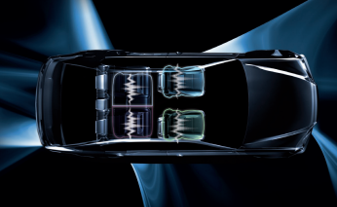
\includegraphics[width=0.7\textwidth]{Img/Chap1/fig1a}
    \caption{This is a car.}
    \label{fig:car}
\end{figure}

subfigure 比较麻烦,实现方法可能会和具体的模板有关。
\begin{figure}[h]
    \centering
    \subfigure[wow]{\label{fig2a}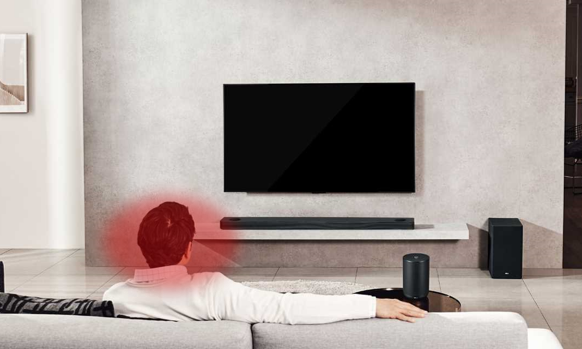
\includegraphics[width=0.31\textwidth]{Img/Chap1/fig1b}}
    ~
    \subfigure[awesome]{\label{fig2b}
\includegraphics[width=0.31\textwidth]{Img/Chap1/fig1c}}
    ~
    \subfigure[]{\label{fig2c}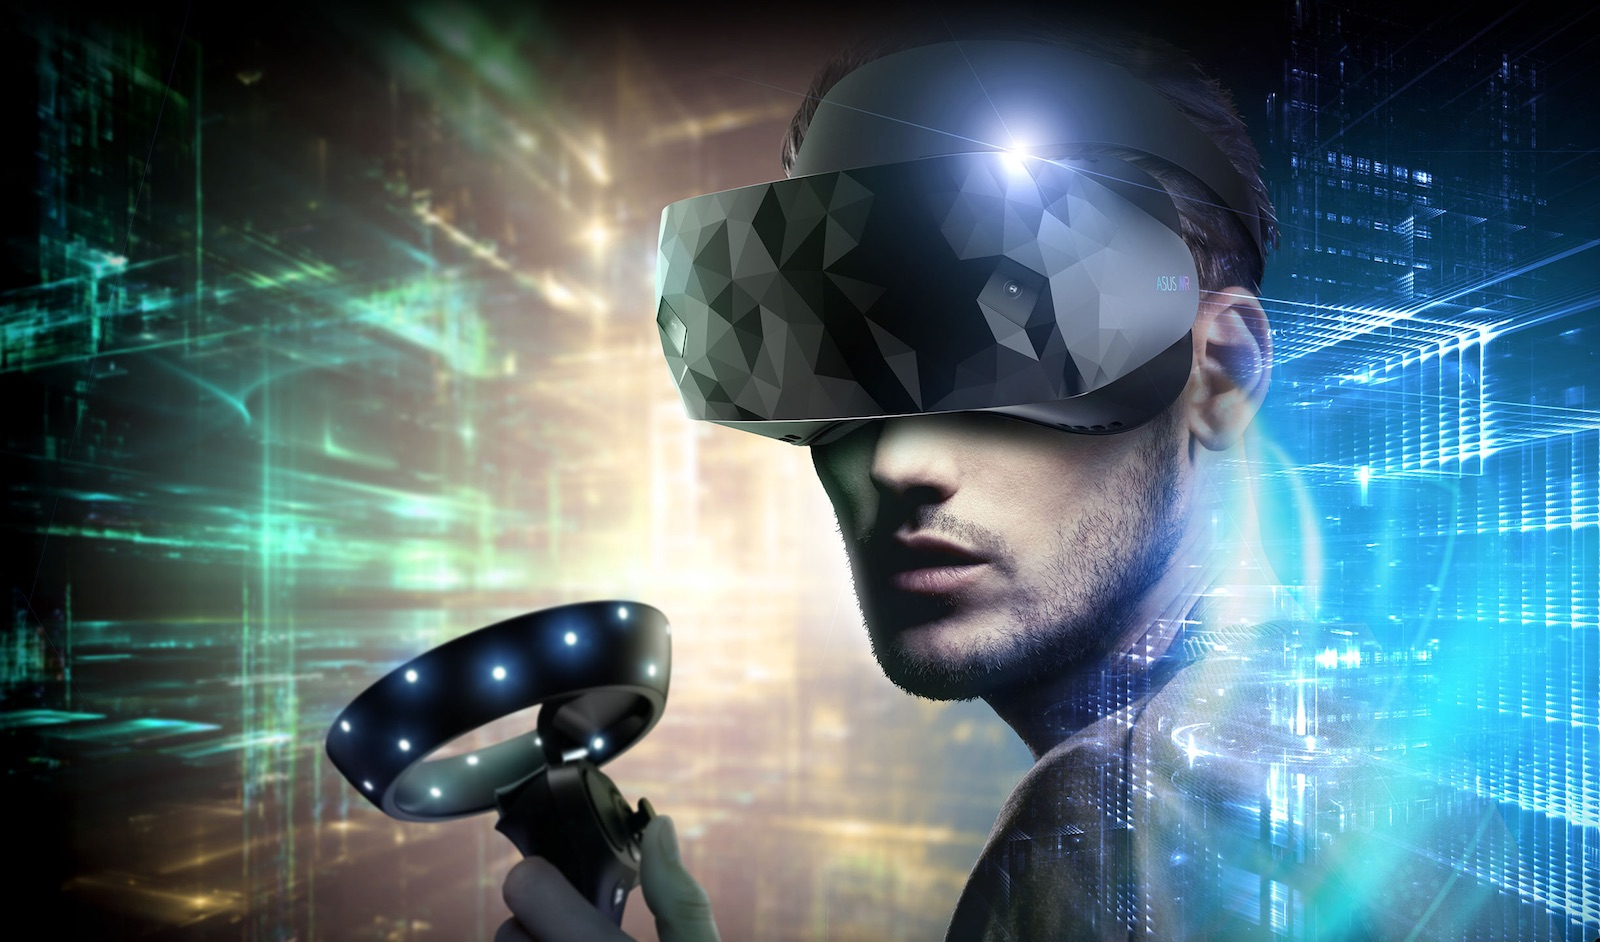
\includegraphics[width=0.31\textwidth]{Img/Chap1/fig1d}}
    \caption{bla bla. (a): wow, (b): awesome, (c):amazing.}
    \label{fig:bla bla}
\end{figure}

% 在这里要空一行,否则下面这段话会和上面那句话混在一起,你可以试试把上面这个空行删掉就知道啥意思了。
我找到 subfigure 的 caption 在哪加了,在\textbackslash subfigure 后面的方括号里面加!
最终是直接在子图下面加注释还是统一在整个 figure 的 caption 里面加注释,还是要看具体期刊的要求。

\subsection{Table}
表格比较麻烦啦。表格的表头是不是要放在表格上面啊,我刚才忘记讲了,一样先打 caption
后面加 label 就好啦,不过如果这个图表以后不需要引用的话,也可以不加 label。

% See \underline{\textcolor{blue}{http://www.tablesgenerator.com/}}
See \url{http://www.tablesgenerator.com/}

\begin{table}[h]
    \centering
    \begin{tabular}{|lcccc|}    % | 表示竖边框
    \hline      % \hline 表示横边框
       & \textbf{PM-1}  & \textbf{PM-2}  & \textbf{MM}    & \textbf{ACC}   \\
    \hline
    AC & 18.02 & 12.05 & 14.42 & 34.01 \\
    AC & 11.46 & 3.85  & 20.45 & 22.73 \\   % 如果最后有 \hline 这里一定要有 \\
    \hline  
    \end{tabular}
    \caption{这里加表头} % 原来是我们大论文的要求表头放上面,latex默认是放下面的,这里放下面就不会间距太小了
    % 如果你也有放上面的需求就告诉我,其实是可以通过加两行代码解决的!
\end{table}

\textbackslash hline 上面必须有两个斜杠来换行,否则会报错!(除了开头的hline)

\section{Tips}

Ctrl + Alt + B ~~ Build 编译 tex % 我把保存自动编译关了,还是手动按编译比较好!

Ctrl + Alt + V ~~ View  预览 pdf

Ctrl + Alt + J ~~ Jump  跳转至 pdf

Ctrl + left click ~~~~ 跳转至源代码

如果报错了一定不要着急,他出错的地方会用红色波浪线标出来的,首先看看报错信息,如果有
``Missing \}" 类似的话,估计是你忘记加大括回了,如果是 ``Undefined control sequence",
那一定是你用了某个命令,缺少相应的宏包,百度一下宏包叫啥然后 usepackage 就好了。
害还不如你直接喊我就完事了!其实你只需要注重论文的内容,排版什么的可以完全交给我来解决。
所以这个 tex 文件里的技巧应该足够你写论文啦。

最后别忘了在 vscode 中修改 json 文件,在文件-首选项-设置中,在右上角找到 打开设置(json),
打开的 json 文件中如果是空的那就直接把我给你的文件复制粘贴进去,如果已经有内容了,那咱就小心点,
把我们文件中最开头的大括号和最后面的大括回删掉,剩下的粘贴到他的 json 文件的末尾。

对了,你 build 的 pdf 文件在根目录下的 Tmp 文件夹下!

\section{Citation}
在 \textbackslash end\{document\} 之前加上最后这两行, bibliographystyle 是指参考文献的格式,
推荐就用 unsrt 吧,按照引用的先后顺序排序,并且按照数字引用。如果你们专业要求
把参考文献按照作者姓名排序,并且用 authoryear 格式引用,那就改成 apalike。

bibliography 里面是你 .bib 文件的文件名,不用加扩展名\cite{Garzone2002Interpretinginthe,Gentzler2017Translationandrewriting,JinYing2018JiaoTiChuan}。

bib 文件中的每一项长这样:

(见源代码中的注释)
% @book{rayleigh1896theory,
%   title={The theory of sound},
%   author={Rayleigh, John William Strutt Baron},
%   volume={2},
%   year={1896},
%   publisher={Macmillan}
% }

book 是这个文献的类型,rayleigh1896theory 叫做 citekey,是你引用时的入口,从谷歌学术中导出的就是\cite{LiYaShu2017KeXueFan}
作者+年份+title的第一个单词,后面的内容就不介绍了,就是这篇文献的基本信息啦。
bib 文件中千万不能有 citekey 相同的文献,会报错的,我就出现过两次找了半天原来是这里出错了!

想要引用的话直接用 \textbackslash cite 命令就可以了,输入完 cite 直接按 Tab
键可以自动补全大括号(begin 等等后面带大括号的一般都可以),然后输入作者的名字+年份
基本就可以筛选出来了,再次按下 Tab 键可以自动补全剩下的 citekey\cite{Malmkjaer2017TheRoutledgeHandbook,Officer1958Introductiontothe,TanXueLan2019DangDaiYi}。

最后差点忘了,刚才视频里忘记说了,你需要下载一个 Zotero 的插件叫做 Better BibTeX,
安装好后在 Zotero 中的编辑-首选项-Better BibTeX 中找到 Citation key format, 
修改为 [auth][year][Title:split-ideographs:select=1,3],这样软件生成的 citekey 就和
谷歌学术中生成的是差不多的了\cite{WangBinHua2019KouYiLi,XuMing2016YiShiChang},
但是不一致哈哈哈!可以从那导出 bibtex 然后导入到 Zotero 库中,我们再 refresh 一下 citekey 就好了。 Test glossary in this page: \gls{mm}, \gls{atf}.

\section{Glossary}
First use: \gls{acc}, second use: \gls{acc}.

First use: \gls{lcmv}. After the first use, you can just type LCMV if you don't want to show the page numbers in the Glossary List.

And other glossary: \gls{fft}, for the second use: \gls{fft}. \Gls{jpvm} you can get an upper-case full name if it's at the beginning of the sentence. \gls{fft}, \gls{mm}, and \gls{atf}.

Massive testing: \Gls{sfr}, \gls{sfs}, \gls{ft}, \gls{pm}, \gls{pc}, \gls{ift}, \gls{isft}, \gls{ifft}, \gls{aed}, \gls{bc}, \gls{wfs}, \gls{hoa}.

\clearpage % 可以强制分页


% !TEX root = ../thesis.tex
%
\chapter{Introduction}
\label{sec:intro}

\cleanchapterquote{You can’t do better design with a computer, but you can speed up your work enormously.}{Wim Crouwel}{(Graphic designer and typographer)}

\Blindtext[2][2]

\section{Postcards: My Address}
\label{sec:intro:address}

\textbf{Ricardo Langner} \\
Alfred-Schrapel-Str. 7 \\
01307 Dresden \\
Germany


\section{Motivation and Problem Statement}
\label{sec:intro:motivation}

\Blindtext[3][1] \cite{Jurgens:2000,Jurgens:1995,Miede:2011,Kohm:2011,Apple:keynote:2010,Apple:numbers:2010,Apple:pages:2010}

\section{Results}
\label{sec:intro:results}

\Blindtext[1][2]

\subsection{Some References}
\label{sec:intro:results:refs}

\cite{WEB:GNU:GPL:2010,WEB:Miede:2011}
\Blindtext[1][1]

\subsubsection{Methodology}
\label{sec:intro:results:refs:method}

\Blindtext[1][2]

\paragraph{Strategy 1}
\Blindtext[1][1]

\begin{lstlisting}[language=Python, caption={This simple helloworld.py file prints Hello World.}\label{lst:pyhelloworld}]
#!/usr/bin/env python
print "Hello World"
\end{lstlisting}

\paragraph{Strategy 2}
\Blindtext[1][1]

\begin{lstlisting}[language=Python, caption={This is a bubble sort function.}\label{lst:pybubblesort}]
#!/usr/bin/env python
def bubble_sort(list):
    for num in range(len(list)-1,0,-1):
        for i in range(num):
            if list[i]>list[i+1]:
                tmp = list[i]
                list[i] = list[i+1]
                list[i+1] = tmp

alist = [34,67,2,4,65,16,17,95,20,31]
bubble_sort(list)
print(list)
\end{lstlisting}

\section{Thesis Structure}
\label{sec:intro:structure}

\textbf{Chapter \ref{sec:related}} \\[0.2em]
\blindtext

\textbf{Chapter \ref{sec:system}} \\[0.2em]
\blindtext

\textbf{Chapter \ref{sec:concepts}} \\[0.2em]
\blindtext

\textbf{Chapter \ref{sec:concepts}} \\[0.2em]
\blindtext

\textbf{Chapter \ref{sec:conclusion}} \\[0.2em]
\blindtext
   % INCLUDE: introduction
\chapter{Related Work}
\label{sec:related}

\cleanchapterquote{A picture is worth a thousand words. An interface is worth a thousand pictures.}{Ben Shneiderman}{(Professor for Computer Science)}

\Blindtext[2][1]

\begin{lstlisting}[language=Java, caption={A simple Hellow World example in Java.}\label{lst:javahelloworld}]
public class HelloWorld {
	public static void main ( String[] args ) {
		// Output Hello World!
		System.out.println( "Hello World!" );
	}
}
\end{lstlisting}

\Blindtext[1][1]

\section{Related Work Section 1}
\label{sec:related:sec1}

\Blindtext[2][2]

\section{Related Work Section 2}
\label{sec:related:sec2}

\Blindtext[3][2]

\section{Related Work Section 3}
\label{sec:related:sec3}

\Blindtext[4][2]

\section{Conclusion}
\label{sec:related:conclusion}

\Blindtext[2][1]
   % INCLUDE: related work

%\part{Additional Example Part}
% % !TEX root = ../thesis.tex
%
\chapter{System}
\label{sec:system}

\cleanchapterquote{Innovation distinguishes between a leader and a follower.}{Steve Jobs}{(CEO Apple Inc.)}

\Blindtext[2][1]

\section{System Section 1}
\label{sec:system:sec1}

\Blindtext[1][2]

\begin{figure}[htb]
	
\includegraphics[width=\textwidth]{Img/Chap2/Clean-Thesis-Figure}
	\caption{Figure example: \textit{(a)} example part one, \textit{(c)} example part two; \textit{(c)} example part three}
	\label{fig:system:example1}
\end{figure}

\Blindtext[1][2]

\section{System Section 2}
\label{sec:system:sec2}

\Blindtext[1][2]

\begin{figure}[htb]
	
\includegraphics[width=\textwidth]{Img/Chap2/Clean-Thesis-Figure}
	\caption{Another Figure example: \textit{(a)} example part one, \textit{(c)} example part two; \textit{(c)} example part three}
	\label{fig:system:example2}
\end{figure}

\Blindtext[2][2]

\section{System Section 3}
\label{sec:system:sec3}

\Blindtext[4][2]

\section{Conclusion}
\label{sec:system:conclusion}

\Blindtext[2][1]
         % INCLUDE: system
% % !TEX root = ../thesis.tex
%
\chapter{Concepts: This text is here to test a very long title, to simulate the line break behavior, to show that an extremely long title also works}
\label{sec:concepts}

\cleanchapterquote{Users do not care about what is inside the box, as long as the box does what they need done.}{Jef Raskin}{about Human Computer Interfaces}

\Blindtext[2][1]

\section{Concepts Section 1}
\label{sec:concepts:sec1}

\Blindtext[2][2]

\section{Concepts Section 2 with a very very long title that illustrates how long section titles are handled in the footer}
\label{sec:concepts:sec2}

\Blindtext[3][2]

\section{Concepts Section 3}
\label{sec:concepts:sec3}

\Blindtext[4][2]

\section{Conclusion}
\label{sec:concepts:conclusion}

\Blindtext[2][1]
       % INCLUDE: concepts
% % !TEX root = ../thesis.tex
%
\chapter{Conclusion}
\label{sec:conclusion}

\Blindtext[2][1]

\section{System Section 1}
\label{sec:conclusion:sec1}

\Blindtext[2][2]

\section{System Section 2}
\label{sec:conclusion:sec2}

\Blindtext[3][2]

\section{Future Work}
\label{sec:conclusion:future}

\Blindtext[2][2]
     % INCLUDE: conclusion

% --------------------------
% Back matter
% --------------------------
%
{%
\setstretch{1.1}
\renewcommand{\bibfont}{\normalfont\small}
\setlength{\biblabelsep}{0pt}
\setlength{\bibitemsep}{0.5\baselineskip plus 0.5\baselineskip}
\printbibliography[nottype=online]
\newrefcontext[labelprefix={@}]
\printbibliography[heading=subbibliography,title={Webpages},type=online]
}
\cleardoublepage

% original places for list of figures, tables and listings

\appendix\cleardoublepage
% !TEX root = ../thesis.tex
%
\chapter{Example Appendix}
\label{sec:appendix}

\Blindtext[1][1]

\section{Appendix Section 1}
\label{sec:appendix:sec1}

\Blindtext[1][1]

\begin{table}[h]
	\begin{tabularx}{\textwidth}{X | X | X}
		%\hline
		Alpha		& Beta			& Gamma			\\ \hline
		0			& 1				& 2				\\ \hline
		3			& 4				& 5				\\ %\hline
	\end{tabularx}
	\label{tab:table1}
	\caption{This is a caption text.}
\end{table}

\section{Appendix Section 2}
\label{sec:appendix:sec2}

\Blindtext[1][1]

\begin{table}[h]
	\begin{tabularx}{\textwidth}{X | X | X}
		%\hline
		Alpha		& Beta			& Gamma			\\ \hline
		0			& 1				& 2				\\ \hline
		3			& 4				& 5				\\ %\hline
	\end{tabularx}
	\label{tab:table2}
	\caption{This is a caption text.}
\end{table}

\Blindtext[1][2]
       % INCLUDE: appendix

\cleardoublepage
% % !TEX root = ../thesis.tex
%
\pagestyle{empty}
\hfill
\vfill
\pdfbookmark[0]{Colophon}{Colophon}
\section*{Colophon}

This thesis was typeset with \LaTeXe.
It uses the \textit{Clean Thesis} style developed by Ricardo Langner.
The design of the \textit{Clean Thesis} style is inspired by user guide documents from Apple Inc.

Download the \textit{Clean Thesis} style at \url{http://cleanthesis.der-ric.de/}.


% \cleardoublepage
% !TEX root = ../thesis.tex
%
%************************************************
% Declaration
%************************************************
\pdfbookmark[0]{Declaration}{Declaration}
\addchap{Declaration}
\label{sec:declaration}
\thispagestyle{empty}

You can put your declaration here, to declare that you have completed your work solely and only with the help of the references you mentioned.

\bigskip

\noindent\textit{\thesisUniversityCity, \thesisDate}

\smallskip

\begin{flushright}
	\begin{minipage}{5cm}
		\rule{\textwidth}{1pt}
		\centering\thesisName
	\end{minipage}
\end{flushright}

%*****************************************
%*****************************************

\clearpage

\newpage
\mbox{}

% **************************************************
% End of Document CONTENT
% **************************************************
\end{document}
